\title{Suscetibilidade Magnética nos Solos Tropicais}
\subtitle{Uma Alternativa Promissora}
\author{por Diego Silva Siqueira e José Marques Jr.}
\maketitle

\section{Suscetibilidade magnética: alternativa para aquisição indireta de informações detalhadas do solo e seus atributos}
\label{sec:1}

A falta de informações detalhadas sobre os recursos do solo é um dos fatores limitantes para o crescimento de diferentes áreas do conhecimento e setores produtivos. Apesar de informações detalhadas dos atributos dos solos serem escassas em território brasileiro, em países como China \citep{liu:2013} e EUA \citep{franze:2006} já são utilizadas nos planejamentos agrícolas e urbanos. Em alguns países da Europa informações da distribuição espacial dos atributos do solo auxiliam na avaliação do impacto da política agrícola em diferentes níveis de detalhe \citep{vandelden:2010}.

\begin{wrapfigure}{l}{0.15\textwidth}
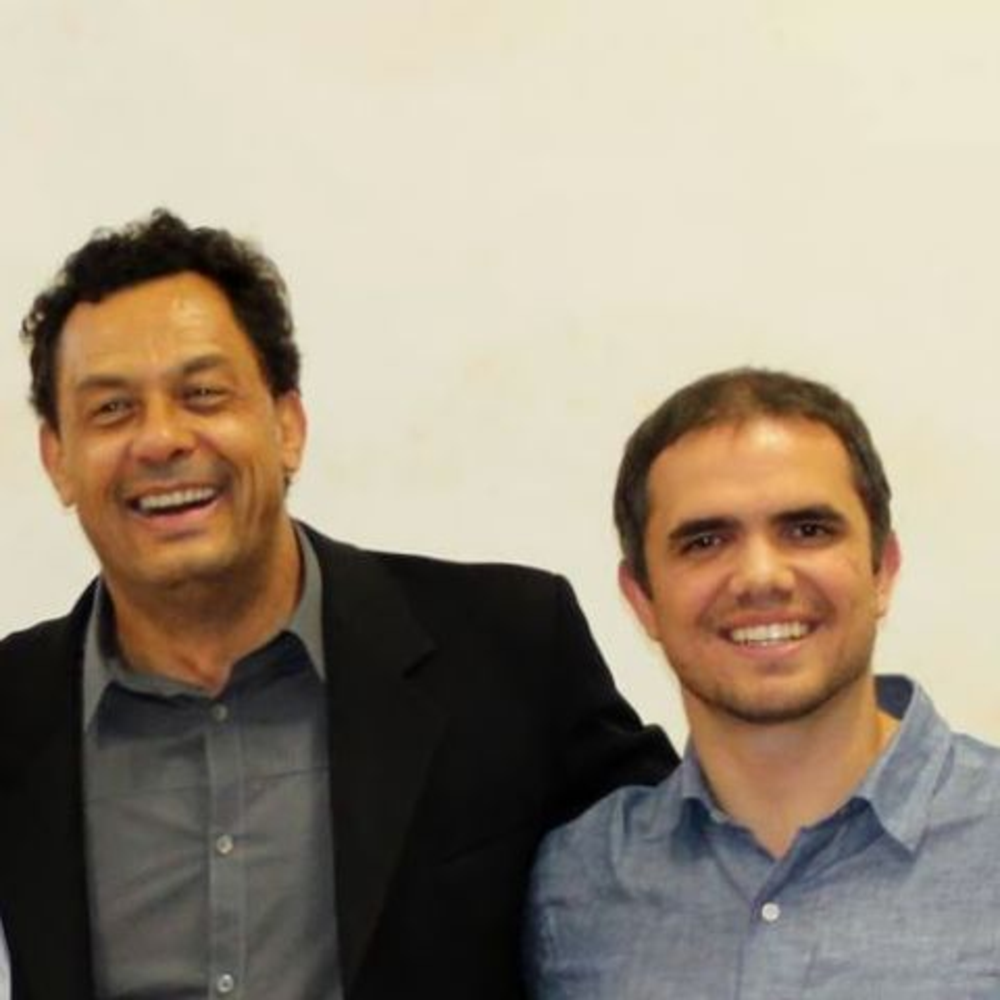
\includegraphics[width=0.15\textwidth]{figuras/foto-diego-junior}
\end{wrapfigure}

Frente às urgências e problemas relacionados à elaboração de um inventário de solos, a caracterização de atributos, pode ser uma alternativa para atender a demanda atual. Essa foi uma das soluções apontadas pelo Painel Técnico Intergovernamental sobre Solos (ITPS, da sigla em inglês) coordenado pela Organização das Nações Unidas para Alimentação e Agricultura (FAO), cujo objetivo é fornecer auxílio técnico e científico em assuntos globais sobre solos e seus atributos, para instituições mundiais ou regionais. Existe, portanto, um alinhamento de propostas sobre o solo e seus atributos para segurança alimentar e a sustentabilidade do planeta.




Porém, para atender a estes e outros objetivos, dois aspectos são fundamentais: - escolha do atributo, que deve ser sensível às variações dos fatores e processo de formação do solo (ex. óxidos de ferro) \citep{camargo:2013}; - ferramentas eficientes para caracterizar a variabilidade destes atributos de maneira precisa e, a baixo custo, viabilizando a caracterização detalhada da variabilidade para grandes áreas. Nesse sentido, destacam-se os avanços tecnológicos relacionados à aquisição de informações sobre os solos utilizando a condutividade elétrica \citep{brennin:2008}, suscetibilidade magnética (SM) \citep{grimley-vepraskas:2000} e espectroscopia de reflectância difusa (ERD) \citep{torrent-barron:1993}.




A condutividade elétrica foi originalmente desenvolvida para regiões temperadas com baixa expressão dos óxidos de ferro. Autores \citep{wu:2008} relatam que essa técnica sofre alterações em regiões com elevada presença de óxidos. Por este motivo, nos solos tropicais, resultados de pesquisas indicam que a SM é uma boa alternativa para identificação de áreas com diferentes padrões de variabilidade \citep{camargo:2013}, bem como na quantificação indireta de atributos físicos, químicos e mineralógicos em áreas com baixo ($Fe_{2}O_{3}<40\text{ g kg}^{-1}$) \citep{siqueira:2010} e alto teor de ferro ($Fe_{2}O_{3}>180\text{ g kg}^{-1}$) \citep{peluco:2013}.




\section{Magnetismo e suscetibilidade magnética: diferença, origem e evolução na Ciência do Solo}
\label{sec:2}




Enquanto o magnetismo está relacionado ao fenômeno de atração ou repulsão, a SM está relacionada com capacidade de um material em magnetizar-se. Mas como os materiais naturais, a exemplo das rochas e minerais se magnetizam?




As rochas podem se magnetizar de diferentes maneiras, a mais comum, é chamada de magnetização termo-remanescente \citep{press:2006}. Porém, antes de esclarecer sobre o processo de magnetização, é preciso conhecer alguns conceitos mineralógicos, como cela unitária. A cela unitária é a menor parte dos minerais presentes nas rochas e nos solos. No centro da cela unitária dos óxidos de ferro, por exemplo, o átomo mais encontrado é o ferro. A magnetização, está relacionada com os elétrons deste átomo. Para saber um pouco mais sobre o assunto "Óxidos de Ferro: Pedoindicadores Ambientais", bem como visualizar figuras e esquemas,recomendamos algumas apresentações do Grupo de Pesquisa CSME (\href{http://www.acervodigital.unesp.br/handle/123456789/40434}{Caracterização do Solo para fins de Manejo Específico}). Retomando, na magnetização termo-remanescente, os elétrons da cela unitária dos minerais magnéticos presentes nas rochas ígneas, orientam-se na direção do campo magnético da Terra na época em que a cela unitária foi formada. Dessa maneira, os minerais ``gravam'' a magnetização do local e da época de formação da rocha. Por este motivo, diz-se que os minerais com capacidade magnética armazenam arquivos naturais contendo registros dos fatores de formação do solo \citep{maher-thompson:1999}, sendo considerados como pedoindicadores. Os minerais também podem adquirir magnetizações posteriores a sua formação, em virtude de processos físicos e químicos. Esse tipo de magnetização é chamado de magnetização remanescente secundária \citep{teixeira:2009}. Para saber um pouco mais sobre magnetismo dos minerais acesse o link \url{http://www.on.br/ead_2012/pdf/modulo2/4_magnetismo_das_rochas.pdf}.




O alinhamento dos elétrons da cela unitária dos minerais, mencionado anteriormente, está relacionado com o spin, que nada mais é do que o movimento de rotação do elétron em um sentido. Quando os elétrons rotacionam em um mesmo sentido, diz-se que há um alinhamento. Conforme descoberto por Hans Christian Orsted em 1820, as correntes elétricas podem criar campos magnéticos. Assim, a movimentação dos elétrons da cela unitária dos minerais, na estrutura cristalina (conjunto de celas unitárias), gera uma microcorrente elétrica, que por sua vez gera um campo magnético. A facilidade com que os elétrons têm de rotacionarem no mesmo sentido (spins pareados), faz com que o campo magnético produzido pelo mineral seja mais forte. Além da distribuição dos elétrons nos subníveis de energia, a direção de cristalização da rede cristalográfica do mineral também interfere em sua SM. Este efeito é conhecido como anisotropia magnética (Figura \ref{fig:figura1}).




\begin{figure*}[tb!]
\begin{minipage}[t]{1\linewidth}
\begin{center}
   \includegraphics[width=\textwidth]{figuras/figura-diego-junior}
   \caption{Diagrama da organização de elétrons do elemento ferro nas celas unitárias do mineral e tipos de suscetibilidade magnética proveniente da rotação dos elétrons (a), intervalo de suscetibilidade magnética para óxidos de ferro puros e rochas (b) (Modificado de DEARING, 1994), variação da suscetibilidade magnética em função da forma e do tamanho do mineral (c) (Modificado de \url{http://www.irm.umn.edu/hg2m/hg2m_c/Image18.gif}, Universidade de Minnesota, Colégio de Ciência e Engenharia) (Extraído de \cite{siqueira:2013})
   \label{fig:figura1}}
\end{center}
\end{minipage}
\end{figure*}




Portanto, a SM de um mineral está relacionada com a rotação dos elétrons da cela unitária dos minerais, presentes na rocha ou no solo \citep{craik:1995}. São considerados 5 tipos básicos de comportamento magnético: diamagnetismo, paramagnetismo, ferromagnetismo, ferrimagnetismo e antiferromagnetismo. Nos minerais diamagnéticos, o número de spins alinhados numa direção é igual ao número de spins na direção oposta, logo os campos magnéticos anulam-se (Exemplo: quartzo). Nos minerais paramagnéticos as camadas eletrônicas estão incompletas. A presença de um campo magnético externo faz com que os spins se alinhem (elétrons giram no mesmo sentido), e mesmo após a retirada do campo magnético, alguns spins permanecem alinhados (Exemplo: olivina). Os minerais ferromagnéticos são um caso especial de paramagnetismo. Após a retirada do campo magnético os spins permanecem alinhados, fazendo com que o mineral possua um grande valor de magnetização remanescente (Exemplo: ferro e cobalto). Nos minerais ferrimagnéticos, os spins não estão emparelhados, assim prevalece a campo magnético resultante do maior número de spins no mesmo sentido (Exemplo: magnetita). Os minerais antiferromagnéticos não apresentam propriedades magnéticas.




Uma situação importante a ser relatada é referente à neosíntese de minerais, especialmente os óxidos de ferro. Quando um ambiente oxídico passa para ambiente redutor, ocorre uma alteração na neosíntese dos minerais, especialmente dos óxidos de ferro. No caso específico dos óxidos, pode ocorrer recristalização dos minerais e o ferro do núcleo da cela unitária, passa de seu estado oxidado ($Fe^{3+}$) para reduzido ($Fe^{2+}$). Com o processo de oxiredução, há nova redistribuição dos elétrons do átomo nas camadas de energia. A nova configuração eletrônica dos elétrons faz com que o número de spins rotacionando em sentidos opostos, seja mais equilibrada, diminuindo o valor da suscetibilidade magnética.




Muitas vezes a SM é confundida com atração magnética. A atração magnética foi utilizada como ferramenta auxiliar de campo nos primeiros levantamentos de solos do Estado de São Paulo na década de 1960 e 1970, para distinguir solos originados de rochas máficas de outros materiais de origem \citep{resende:1988}.




Nos solos originados de rochas máficas (ricos em magnetita e maghemita), quando um ímã qualquer é aproximado da superfície do solo, há atração entre suas partículas e o ímã, e o solo prende-se ao ímã. Portanto, a atração magnética pode ser interpretada como ferramenta qualitativa. No campo, os mapeadores notaram que, mesmo tratando-se de um solo originado de rocha máfica, havia diferentes intensidades de atração magnética. Em alguns locais, a superfície do ímã ficava mais recoberta por partículas de solo e, em outros locais, menos recoberta. Isso inspirou a aplicação da atração magnética como ferramenta quantitativa e estudos sobre a SM.




Porém, devido à dificuldade de reprodução dos resultados e à baixa exatidão entre os laboratórios para expressar as diferentes interações magnéticas das amostras de solo, a técnica caiu em desuso \citep{resende:1988}. Com os avanços dos sensores e de técnicas alternativas na avaliação da interação magnética \citep{carneiro:2003}, o uso da SM como ferramenta auxiliar na caracterização quantitativa da variabilidade de campo \citep{santos:2013} ganha novas expectativas.




Um dos equipamentos mais utilizados para avaliação da SM é o sensor da Bartington MS2, acoplado ao sensor Bartington MS2B. A avaliação pode ser feita no campo, em laboratório, em amostras de terra fina seca ao ar (TFSA) ou fração argila, silte e areia. Para aplicações em estudos de pedometria, com foco no desenvolvimento de funções de pedotransferência para quantificação, recomenda-se que sejam feitas avaliações em baixa frequência (0,47 kHz) \citep{dearing:1994}. Segundo estes autores, as medições de dupla frequência (alta – 4,7 kHz e baixa) devem ser utilizadas em estudo de caráter qualitativo para indicar a presença de minerais magnéticos de domínio simples, múltiplos e anisotropia magnética. Uma alternativa prática e barata para avaliação da SM é a utilização de uma balança analítica. Os resultados de SM, obtidos pela adaptação da balança, tiveram boa correlação ($R^{2}=0,942;\,P<0,01$) com os resultados obtidos pelo sensor da Bartington \citep{siqueira:2010}.




No sensoriamento remoto, o magnetismo e SM são utilizados rotineiramente como ferramenta, no detalhamento do mapa geológico \citep{ruy:2006} e recentemente no desenvolvimento de assinaturas geomagnéticas, para estudos detalhados sobre os solos da China \citep{xia:2007}. A vantagem em se utilizar informações geofísicas, está relacionada ao seu potencial para descrever processos de formação do solo, os quais dificilmente alteram-se em curto prazo por intermédio de ações antrópicas. A mineralogia do solo é um dos principais indicadores da variação destes processos pedogenéticos \citep{camargo:2013}. Como a SM é produto da variação dos minerais presentes do solo \citep{siqueira:2013}, podemos inferir que o mapa da SM expressa o mapa dos processos pedogenéticos do solo.




As aplicações do conhecimento sobre geofísica, especificamente do magnetismo, podem ser associadas à habilidade das áreas em explorar a multidisciplinaridade. Fazendo uma comparação das publicações com o termo ``\textit{magnetism}'', na base referencial multidisciplinar, Web of Science, entre as áreas Agronomia e Mineralogia, versos Ciências Ambientais e Ecologia, nota-se que, nas áreas Agronomia e Mineralogia, não houve aumento no número de publicações em 2013 (5 publicações) em comparação ao ano de 1997 (5 publicações). Em contra partida, na área de Ciências Ambientais e Ecologia, houve um aumento de 433\%, de 2013 (16 publicações) em comparação ao ano de 1997 (3 publicações). Este fato exemplifica a importância da multidisciplinaridade e corrobora relatos de pesquisadores brasileiros, a exemplo \cite{vidal-torrado:2005}, e estrangeiros, a exemplo \cite{grunwald:2011}, sobre a formação e educação do moderno cientista do solo, cuja reflexão é ``\textit{O quão multidisciplinar devemos ser frente aos desafios}?''.




\begin{footnotesize}
\begin{thebibliography}{99}




\bibitem[Brenning et~al.(2008)]{brennin:2008}
Brenning, A., Koszinski, S., Sommer, M. (2008)
\newblock Geostatistical homogenization of soil conductivity across field boundaries.
\newblock {\em Geoderma} 143: 254-260.




\bibitem[Camargo et~al.(2010)]{camargo:2010}
Camargo, L. A., Marques Jr., J., Pereira, G. T. (2010)
\newblock Spatial variability of physical attributes of an Alfisol under different hillslope curvatures.
\newblock {\em Revista Brasileira de Ciência do Solo} 34: 617-630.




\bibitem[Camargo(2013)]{camargo:2013}
Camargo, L. A. (2013)
\newblock Mineralogia da argila por difração de raios x e espectroscopia de reflectância difusa em Latossolos sob diferentes superfícies geomórficas.
\newblock {\em Tese (Doutorado) – Faculdade de Ciências Agrárias e Veterinárias, Universidade Estadual Paulista, Jaboticabal} 2013.




\bibitem[Carneiro et~al.(2003)]{carneiro:2003}
Carneiro, A. A. O., Touso, A. T., Baffa, O. (2003)
\newblock Avaliação da suscetibilidade magnética usando uma balança analítica.
\newblock {\em Química Nova} 26: 952-956.




\bibitem[Craik(1995)]{craik:1995}
Craik, D. (1995)
\newblock Magnetism, Principles and Aplications.
\newblock {\em John Wiley and Sons} p.1-459.




\bibitem[Dearing(1994)]{dearing:1994}
Dearing, J.A. (1994)
\newblock Environmental magnetic susceptibility. Using the Bartington MS2 system.
\newblock {\em England: British Library} 104 p. Disponível em: \url{http://gmw.com/magnetic\_properties/pdf/Om0409\%20J\_Dearing\_Handbook_iss7.pdf}.




\bibitem[Franze et~al.(2006)]{franze:2006}
Franzen, D. W., Nanna, T., Norvell, W. A. (2006)
\newblock A Survey of Soil Attributes in North Dakota by Landscape Position.
\newblock {\em Agronomy Journal} 98: 1015-1022.




\bibitem[Grimley e Vepraskas(2000)]{grimley-vepraskas:2000}
Grimley, D. A., Vepraskas, M. J. (2000)
\newblock Magnetic susceptibility for use in delineating hydric soils.
\newblock {\em Soil Science Society American Journal} 64: 2174-2180.




\bibitem[Grunwald et~al.(2011)]{grunwald:2011}
Grunwald, S., Thompson, J. A., Boettinger, J. L. (2011)
\newblock Digital Soil Mapping and Modeling at Continental Scales: Finding Solutions for Global Issues.
\newblock {\em Soil Science Society American Journal} 75: 1201-1213.




\bibitem[Liu et~al.(2013)]{liu:2013}
Liu, Y., Lv, J., Zhang, B., Bi, J. (2013)
\newblock Spatial multi-scale variability of soil nutrients in relation to environmental factors in a typical agricultural region, Eastern China.
\newblock {\em Science of the Total Environment} p. 108-119.




\bibitem[Maher e Thompson(1999)]{maher-thompson:1999}
Maher, B. A., Thompson, R. (1999)
\newblock Palaeomonsoons I: the magnetic record of palaeoclimate in the terrestrial loess and palaeosol sequences, in quaternary climates, environments and magnetism.
\newblock {\em Cambridge: University Press} p. 81–125.




\bibitem[Peluco et~al.(2013)]{peluco:2013}
Peluco, R. G., Marques Jr., Siqueira, D. S., Pereira, G. T., Barbosa, R. S., Teixeira, D. B., Adame, C. R., Cortez, L. A. (2013)
\newblock Suscetibilidade magnética do solo e estimação da capacidade de suporte à aplicação de vinhaça.
\newblock {\em Pesquisa Agropecuária Brasileira} 48:661-672.




\bibitem[Press et~al.(2006)]{press:2006}
Press, F., Siever, R., Grotzinger, J., Jordan, T. H. (2006)
\newblock Para entender a Terra. 4ª edição. Versão traduzida
\newblock {\em Bookman} p. 656.




\bibitem[Resende et~al.(1988)]{resende:1988}
Resende, M., Santana, D. P., Rezende, S. B. (1988)
\newblock Susceptibilidade magnética em Latossolo do Sudeste e Sul do Brasil.
\newblock {\em In: REUNIÃO DE CLASSIFICAÇÃO, CORRELAÇÃO DE SOLOS E INTERPRETAÇÃO DE APTIDÃO AGRÍCOLA, Rio de Janeiro, EMBRAPA-SNLCS/SBCS} p 233–258.




\bibitem[Ruy et~al.(2006)]{ruy:2006}
Ruy, A. C., Silva, A. M., Toledo, C. L. B.,Souza Filho, C. R. (2006)
\newblock Uso de dados aerogeofísicos de alta densidade para mapeamento geológico em terrenos altamente intemperizados: o estudo de caso da Região de Cláudio, porção Sul do Cráton São Francisco.
\newblock {\em Revista Brasileira de Geofísica} 24:535-546.




\bibitem[Santos et~al.(2013)]{santos:2013}
Santos, H. L., Marques Jr., J., Matias, S. S. R., Siqueira, D. S., Pereira, G. T. (2013)
\newblock Erosion factors and magnetic susceptibility in differet compartments of a slope in Gilbués-PI, Brazil.
\newblock {\em Engenharia Agrícola} 33:64-74.




\bibitem[Siqueira et~al.(2010)]{siqueira:2010}
Siqueira, D. S., Marques Jr., J., Matias, S. S. R., Barrón, V., Torrent, J., Baffa, O., Oliveira, L. C.  (2010)
\newblock Correlation of properties of Brazilian Haplustalfs with magnetic susceptibility measurements.
\newblock {\em Soil, Use and Management} 26:425-431.




\bibitem[Siqueira(2013)]{siqueira:2013}
Siqueira, D. S. (2013)
\newblock Mapeamento detalhado e planejamento amostral para Latossolos utilizando suscetibilidade magnética e cor no contexto da relação solo-paisagem.
\newblock {\em Tese (Doutorado) – Faculdade de Ciências Agrárias e Veterinárias, Universidade Estadual Paulista, Jaboticabal} 2013.




\bibitem[Teixeira et~al.(2009)]{teixeira:2009}
Teixeira, W., Toledo, M. C. M. De, Fairchild, T. R., Taioli, F. (2009)
\newblock Decifrando a Terra.São Paulo.
\newblock {\em Oficina de Textos} p.557.




\bibitem[Torrent e Barrón(1993)]{torrent-barron:1993}
Torrent, J., Barrón, V. (1993)
\newblock Laboratory measurements of soil color: theory and practice
\newblock {\em In: BIGHAM, J. M., CIOLKOSZ, E. J. (Ed) Soil Color. Soil Science Society of America, Special Publication} p. 21-33.




\bibitem[Van Delden et~al.(2010)]{vandelden:2010}
Van Delden, H., Stuczynski, T., Ciaian, P., Paracchini, M. L., Hurkens, J., Lopatka, A., Shi, Y., Gomez Prieto, O., Calvo, S., Van Vliet, J., Vanhout, R. (2010)
\newblock Integrated assessment of agricultural policies with dynamic land use change modelling.
\newblock {\em Ecological Modelling} 221:2153–2166.




\bibitem[Vidal-Torrado et~al.(2005)]{vidal-torrado:2005}
Vidal-Torrado, P., Lepsch, I. F., Castro, S. S. (2005)
\newblock Laboratory measurements of soil color: theory and practice
\newblock {\em In: P. Vidal-Torrado, Luiz R. Ferraciu, M. Cooper, Elke J. Cardoso, Luiz I. Prochonow. (Org.). Tópicos em Ciência do Solo. Viçosa: Sociedade Brasileira de Ciência do Solo} 4:145-192.




\bibitem[Wu et~al.(2008)]{wu:2008}
Wu,Y.; Slater, L.;  Versteeg, R.;  Labrecque, D. (2008)
\newblock A comparison of the low frequency electrical signatures of iron oxide versus calcite precipitation in granular zero valent iron columns.
\newblock {\em Journal of Contaminant Hydrology} 95:154–167.




\bibitem[Xia et~al.(2007)]{xia:2007}
Xia, D., Jin, M., Liu X., Chen F., Ma J., Zhao H., Wang X., Wei H. (2007)
\newblock A preliminary study on the magnetic signatures of modern soil in Central Asia.
\newblock {\em Frontiers of Earth Science} 1:275–283.

\end{thebibliography}
\end{footnotesize}

\address{Diego Silva Siqueira\\
  \begin{footnotesize}
    UNESP Câmpus de Jaboticabal - Grupo de Pesquisa CSME\\
    \url{http://lattes.cnpq.br/8836609544198735}\\
    \email{diego\_silvasiqueira@yahoo.com.br}
  \end{footnotesize}
}\\
\vskip
\address{José Marques Jr.\\
  \begin{footnotesize}
    UNESP Câmpus de Jaboticabal - Grupo de Pesquisa CSME\\
    \url{http://lattes.cnpq.br/5425582467938015}\\
    \email{marques@fcav.unesp.br}
  \end{footnotesize}
}
%%% Local Variables:
%%% mode: latex
%%% TeX-master: 3rd-edition.tex
%%% End: